\documentclass[10pt,leqno]{amsart}
\usepackage{graphicx}
\baselineskip=16pt

\usepackage{indentfirst,csquotes}
\usepackage{here}

\topmargin= .5cm
\textheight= 20cm
\textwidth= 32cc
\baselineskip=16pt

\evensidemargin= .9cm
\oddsidemargin= .9cm

\usepackage{amssymb,amsthm,amsmath}
\usepackage{xcolor,paralist,hyperref,fancyhdr,etoolbox}
\usepackage{letltxmacro}
\newtheorem{theorem}{Theorem}[]
\newtheorem{definition}[theorem]{Definition}
\newtheorem{example}[theorem]{Example}
\newtheorem{lemma}[theorem]{Lemma}
\newtheorem{proposition}[theorem]{Proposition}
\newtheorem{corollary}[theorem]{Corollary}
\newtheorem{conjecture}[theorem]{Conjecture}

\hypersetup{ colorlinks=true, linkcolor=black, filecolor=black, urlcolor=blue }
\def\proof{\noindent {\it Proof. $\, $}}
\def\endproof{\hfill $\Box$ \vskip 5 pt }

\LetLtxMacro{\oldincludegraphics}{\includegraphics}
\renewcommand{\includegraphics}[2][]{%
  \IfFileExists{#2}{\oldincludegraphics[#1]{#2}}{\fbox{Missing figure}}%
}

\begin{document}

\begin{titlepage}
\centering
\vspace*{2cm}

{\LARGE \bfseries A3 High Energy Physics Coursework Experiment Report\par}

\vspace{1.5cm}

{\large Baiyuan Chen\par}
\vspace{0.3cm}
{\large CRSID: bc654\par}
\vspace{0.3cm}
{\large bc654@cam.ac.uk\par}

\vspace{1.5cm}

{\large Word Count: $\sim$1327\par}

\vspace{1.5cm}

{\large MPhil in Data Intensive Science\par}
\vspace{0.3cm}
{\large University of Cambridge\par}
\vspace{1.5cm}

{\small\textit{Below, ``we'' is used instead of ``I'' to follow the convention of scientific writing.}\par}

\vfill
\end{titlepage}

\section{Introduction (184 words)}

The decay $B_s^0 \to K^+\pi^-K^-\pi^+$ proceeds predominantly through the intermediate resonant channel $B_s^0 \to K^{*0}(892)\bar{K}^{*0}(892)$, where each $K^{*0}$ decays to a $K\pi$ pair. This charmless four-body decay is mediated by $b \to d$ loop (penguin) and tree-level transitions, making it sensitive to CP violation and potential contributions from physics beyond the Standard Model~\cite{lhcb_kskpi}.

The angular structure of the $K^{*0}\bar{K}^{*0}$ system provides access to polarisation amplitudes, which encode information about the underlying weak decay dynamics. Measurements by the LHCb collaboration have established the branching fraction and performed amplitude analyses of related $B_s^0$ decay modes involving $K\pi$ pairs~\cite{lhcb_kskpi}. Higher $K\pi$ resonances such as the $K_2^*(1430)$ and the scalar $K_0^*(1430)$ are also expected to contribute to the four-body final state, complicating the resonant substructure.

In this analysis, we isolate the $B_s^0 \to K^+\pi^-K^-\pi^+$ signal from data containing ${\sim}939{,}000$ candidates using a multivariate classifier, particle identification (PID) cuts, and invariant-mass vetoes. We then perform a mass fit and use the sPlot technique~\cite{splot} to project the signal into intermediate $K\pi$ invariant masses and identify resonant contributions. The Monte Carlo (MC) simulation sample contains ${\sim}5.4$ million events with per-event weights correcting for simulation--data discrepancies.


\section{Reducing combinatorial background (408 words)}

Combinatorial background arises from random $K^+\pi^-K^-\pi^+$ combinations that do not originate from a genuine $B$ meson decay. We train a gradient-boosted decision tree (XGBoost BDT) to separate signal from this background.

\textbf{Training samples.} Signal is taken from the MC simulation sample with per-event simulation weights applied during training; background from data events in the upper $B_s^0$-mass sideband ($m_{B_s} > 5600$~MeV/$c^2$), which lies well above the $B_s^0$ peak and is dominated by combinatorial events.

\textbf{Feature selection.} We exclude all invariant mass variables ($B_s^0$, $K^*$, single-track masses) to avoid biasing the subsequent mass fit, and exclude vertex position coordinates ($x, y, z$) as these are detector-specific and may cause the model overly fit. The remaining 97 common branches are ranked by the two-sample Kolmogorov--Smirnov (KS) statistic between signal and background; the top 20 features are selected, dominated by flight distance significance, impact parameter variables, and the cosine of the momentum--decay-angle. The signal sample is downsampled to 150{,}000 events to approximately balance the class sizes, and the combined sample is split 50/50 into training and test sets.

\textbf{Classifier and hyperparameters.} We use an XGBoost BDT with conservative hyperparameters: \texttt{max\_depth=2}, \texttt{min\_child\_weight=100}, \texttt{learning\_rate=0.1}, \texttt{subsample=0.8}, and 400 boosting rounds. The shallow tree depth and large minimum child weight regularise the model and limit overtraining. The classifier achieves a ROC AUC of 0.992 on the training set and 0.991 on the test set. An overtraining check comparing the BDT output distributions between training and test samples for both classes (Figure~\ref{fig:bdt_overtrain}) shows good agreement, with most pull values consistent with statistical fluctuations within the $\pm 2\sigma$ band.

\begin{figure}[htbp]
\centering
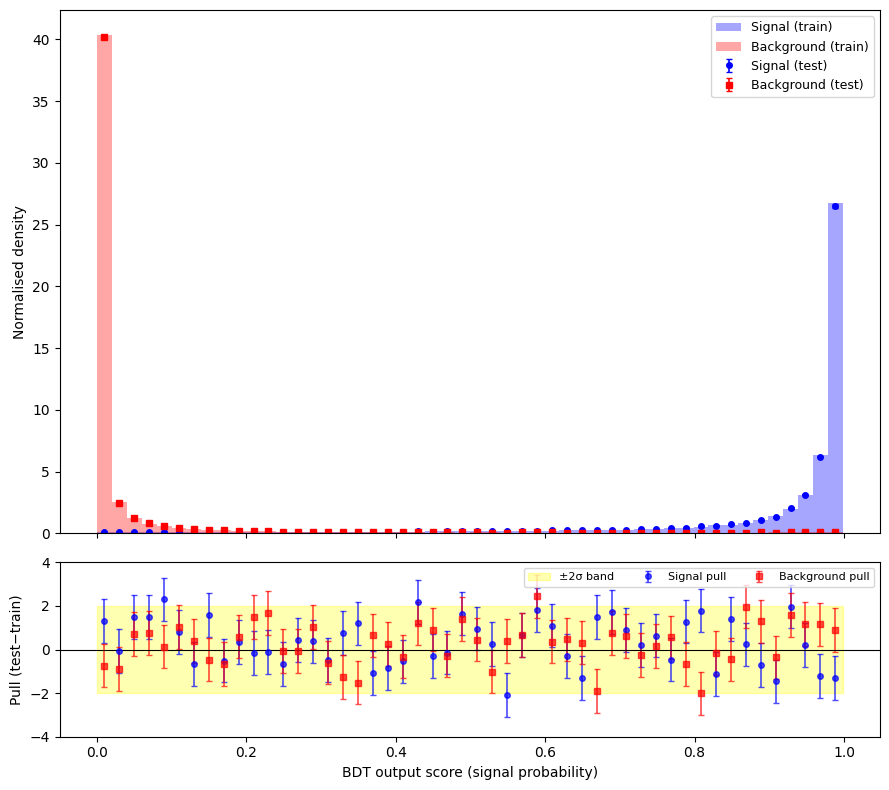
\includegraphics[width=0.6\textwidth]{../figures/exp_q2_bdt_overtrain.png}
\caption{BDT output distributions (left) and test--train pull (right) for signal and background.}
\label{fig:bdt_overtrain}
\end{figure}

\textbf{Optimal cut.} We scanned BDT output thresholds and evaluated
$S/\sqrt{S+B}$ at each working point. The background yield $B$ in the
signal window ($5340 < m_{B_s} < 5400$~MeV, width 60~MeV) was estimated
by counting events in mass sidebands
$[5150, 5300] \cup [5450, 5750]$~MeV (total width 450~MeV) and scaling
by the ratio $60/450$; the signal yield was then obtained as
$S = N_{\text{window}} - B$.  The resulting significance curve
(Figure~\ref{fig:bdt_opt}) peaks at a BDT score of $0.088$, giving
$S/\sqrt{S+B} = 212.2$ and retaining 291{,}407 events (31.0\%).  The
$m_{B_s}$ distribution after this cut (Figure~\ref{fig:mass_bdt}) shows
a prominent $B_s^0$ peak with substantially reduced smooth background,
though several peaking structures remain.

\begin{figure}[htbp]
\centering
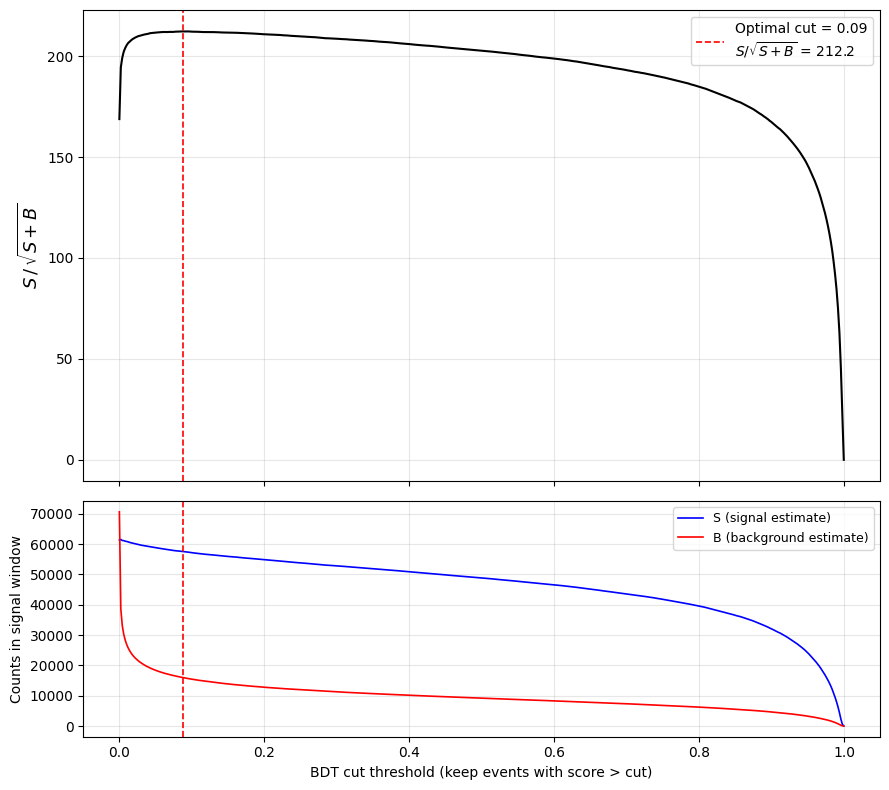
\includegraphics[width=0.5\textwidth]{../figures/exp_q2_bdt_significance.png}
\caption{$S/\sqrt{S+B}$ as a function of BDT cut threshold; the dashed line marks the optimum.}
\label{fig:bdt_opt}
\end{figure}

\begin{figure}[htbp]
\centering
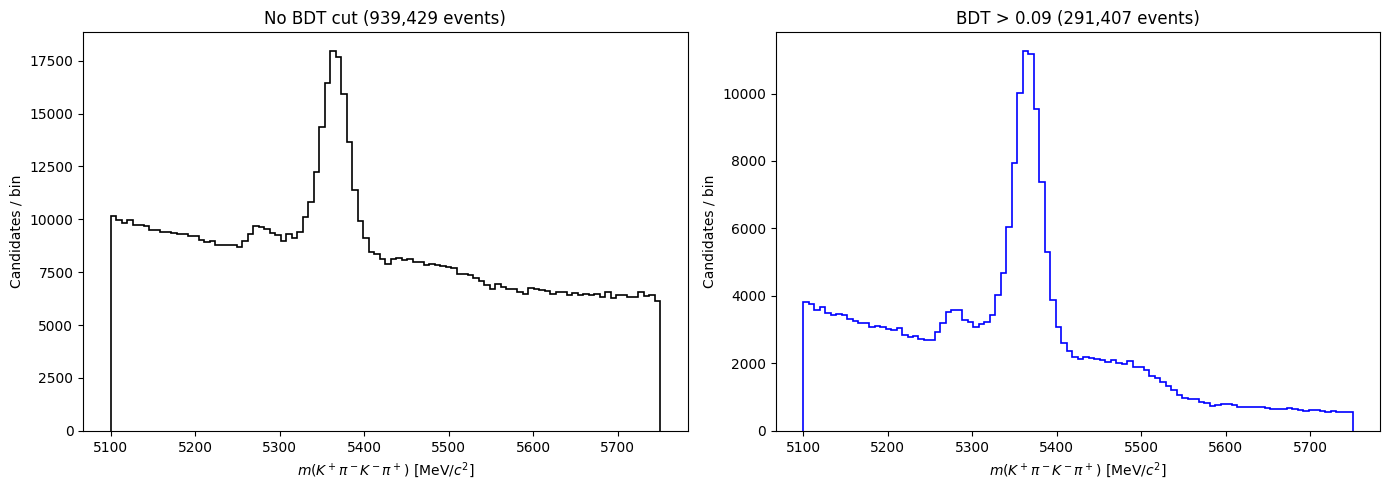
\includegraphics[width=0.95\textwidth]{../figures/exp_q2_mass_bdt_cut.png}
\caption{$m(K^+\pi^-K^-\pi^+)$ before (left) and after (right) the optimal BDT cut.}
\label{fig:mass_bdt}
\end{figure}


\section{Reducing other backgrounds (312 words)}

After the BDT cut, peaking backgrounds from specific $B$ decays with misidentified tracks remain. We address these using PID cuts and invariant-mass vetoes.

\textbf{Identifying misidentification backgrounds.}
We recompute two-body invariant masses under swapped mass hypotheses 
(Figure~\ref{fig:swap_mass}). Assigning the kaon mass to each pion 
reveals a sharp spike at the $\phi(1020)$ mass in both $m(K^+, \pi^- \!\to\! K)$ 
and $m(K^-, \pi^+ \!\to\! K)$, confirming contamination from $B_s^0 \to \phi K^{*0}$ 
where a kaon from $\phi \to K^+K^-$ is misreconstructed as a pion. 
The misassignment of a lighter pion mass to a true kaon shifts the 
reconstructed $B_s^0$ mass upward, creating the broad shoulder above 
the signal peak visible in Figure~\ref{fig:mass_bdt}. Swapping 
$K \to \pi$ produces a broad enhancement near the $\rho(770)$ region 
but no sharp peak, indicating negligible $B \to \rho^0\rho^0$ 
contamination. The $\pi \to p$ distributions are featureless, 
suggesting no meaningful $\Lambda_b$ contamination.

\begin{figure}[htbp]
\centering
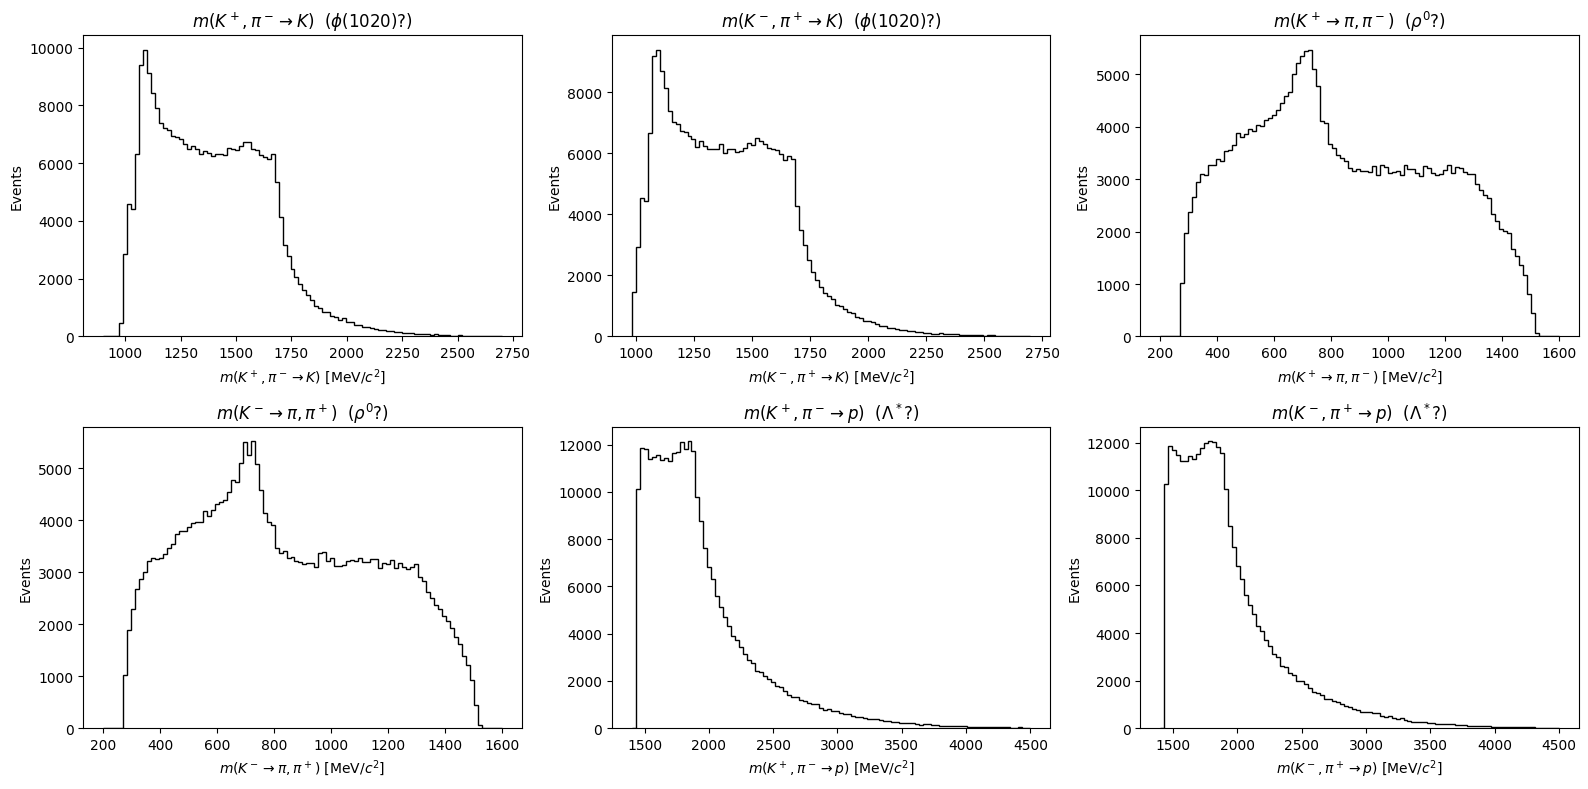
\includegraphics[width=0.95\textwidth]{../figures/exp_q3_swap_mass.png}
\caption{Swapped-mass distributions: $\pi \to K$ (top left/centre), $K \to \pi$ (top right, bottom left), and $\pi \to p$ (bottom centre/right).}
\label{fig:swap_mass}
\end{figure}

\textbf{PID cuts.}
Sideband-based $S/\sqrt{S+B}$ is inappropriate for peaking backgrounds, 
which sit under the signal peak and are counted as ``signal'' in 
sideband subtraction. Instead, we monitor the contamination ratio 
$N_{B^0\text{ region}}/N_{B_s\text{ region}}$ (using mass windows 
$5250$--$5310$ and $5340$--$5400$~MeV) alongside signal efficiency as 
a function of PID threshold (Figure~\ref{fig:pid_opt}). We choose 
$\texttt{ProbNNk} > 0.25$ for both kaons and $\texttt{ProbNNpi} > 0.15$ 
for both pions, balancing contamination reduction against signal 
efficiency (${\sim}83\%$ and ${\sim}98\%$ respectively).

\begin{figure}[htbp]
\centering
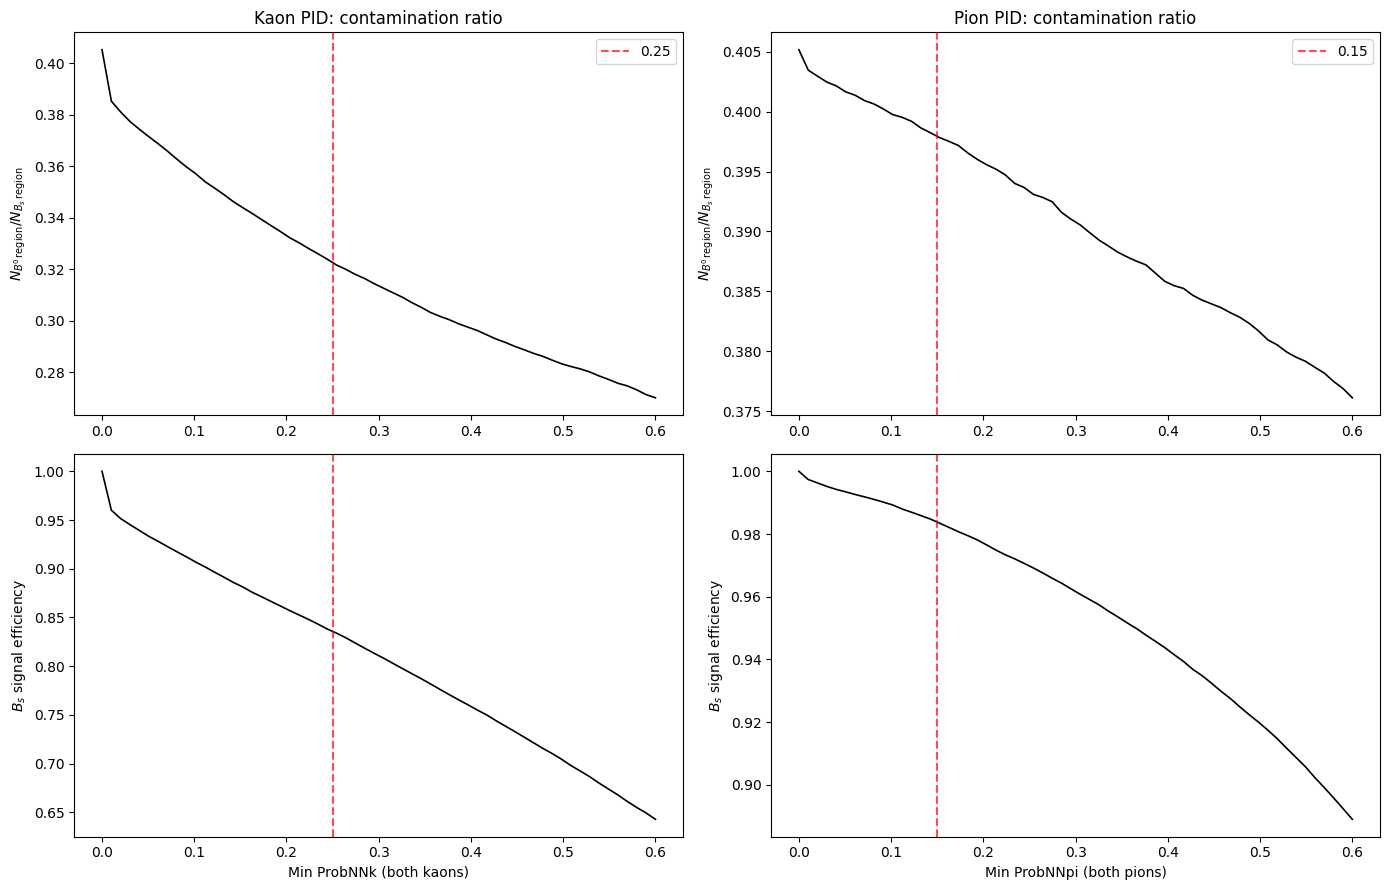
\includegraphics[width=0.8\textwidth]{../figures/exp_q3_pid_opt.png}
\caption{Contamination ratio (top) and signal efficiency (bottom) vs.\ PID threshold for kaons (left) and pions (right).}
\label{fig:pid_opt}
\end{figure}

\textbf{Mass vetoes.}
Events with $m(K^+, \pi^- \!\to\! K)$ or $m(K^-, \pi^+ \!\to\! K)$ within $[1005, 1035]$~MeV are vetoed, directly removing the $\phi(1020)$-fed contamination.

After all cuts, 175{,}726 events remain (Figure~\ref{fig:mass_final}). 
The $B^0 \to K^+\pi^-K^-\pi^+$ peak at ${\sim}5280$~MeV (same final 
state, irreducible by PID) and the partially reconstructed hump below 
${\sim}5220$~MeV (e.g.\ $B_s \to D_s^- K^{*+}$ with a missing 
particle) cannot be removed by cuts and are modelled in the mass fit.

\begin{figure}[htbp]
\centering
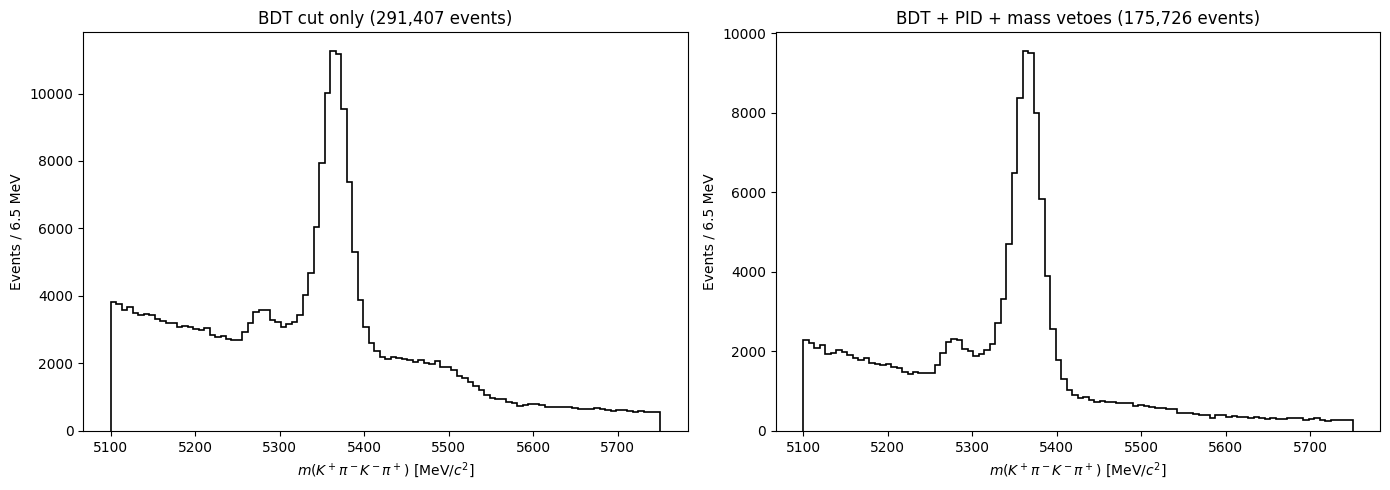
\includegraphics[width=0.95\textwidth]{../figures/exp_q3_mass_final.png}
\caption{$m_{B_s}$ after BDT cut only (left) and after BDT $+$ PID $+$ mass vetoes (right).}
\label{fig:mass_final}
\end{figure}


\section{$B$ candidate mass fit (153 words)}

We perform a binned extended maximum-likelihood fit to $m(K^+\pi^-K^-\pi^+)$ in the range $5200$--$5750$~MeV (130 bins of 4.2~MeV) using \texttt{iminuit}~\cite{iminuit} with an \texttt{ExtendedBinnedNLL} cost function. Three components are included:

\begin{enumerate}
\item \textbf{$B_s^0$ signal}: double Gaussian with shared mean $\mu_{B_s}$, core width $\sigma_1$, wide width $r_\sigma \cdot \sigma_1$, and core fraction $f_\text{core}$. All shape and yield parameters float.

\item \textbf{$B^0 \to K^+\pi^-K^-\pi^+$}: single Gaussian with floating mean $\mu_{B^0}$ and width tied to $\sigma_1$ (same detector resolution). Yield floats.

\item \textbf{Combinatorial}: exponential $e^{\alpha m}$ with slope $\alpha < 0$ floating. The fit range begins at 5200~MeV to avoid the partially reconstructed region.
\end{enumerate}

The fit (Figure~\ref{fig:mass_fit}) converges with yields $N_{B_s} = 61{,}629 \pm 561$, $N_{B^0} = 6{,}840 \pm 196$, and $N_\text{comb} = 59{,}955 \pm 571$. The $B_s^0$ mass is $5365.0 \pm 0.1$~MeV/$c^2$ with core resolution $\sigma_1 = 17.2 \pm 0.1$~MeV/$c^2$. The $B^0$ mass is fitted at $5288.2 \pm 0.6$~MeV/$c^2$. Pull distributions are consistent with zero across the fit range.

\begin{figure}[htbp]
\centering
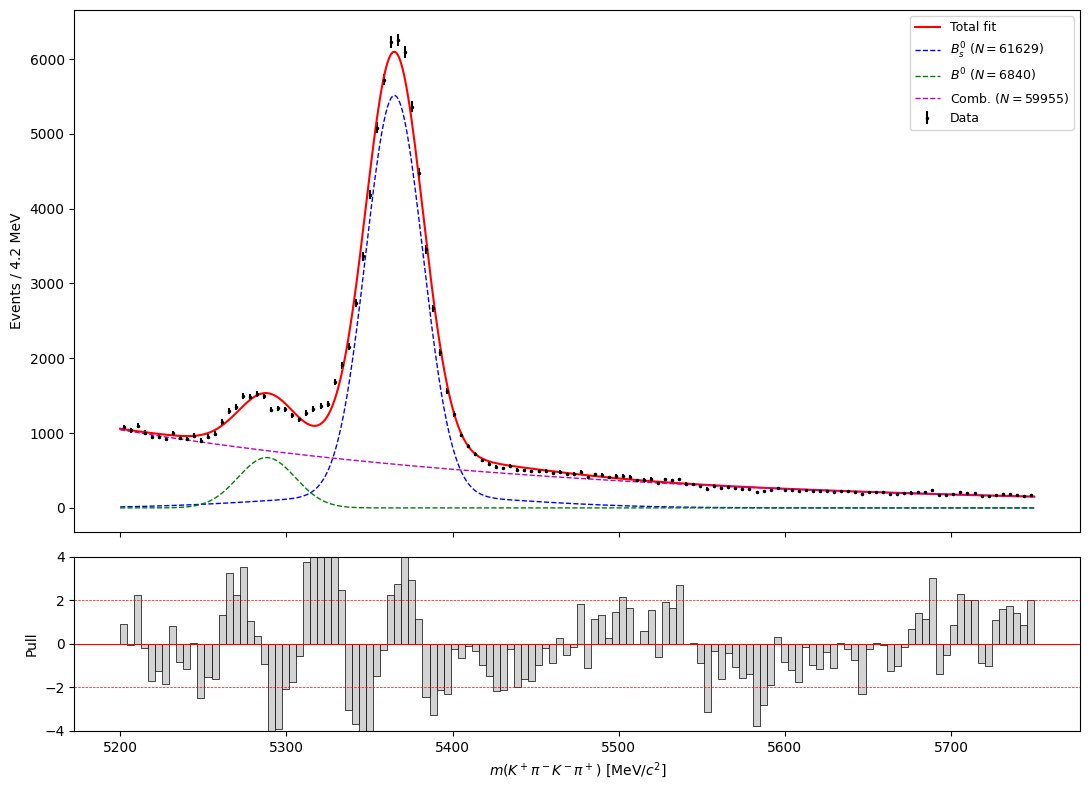
\includegraphics[width=0.75\textwidth]{../figures/exp_q4_mass_fit.png}
\caption{$B$ candidate mass fit with individual components overlaid (top) and pull distribution (bottom).}
\label{fig:mass_fit}
\end{figure}

\section{Projection of the signal component in intermediate masses (208 words)}

We use the sPlot technique~\cite{splot} to compute per-event signal
sWeights from the mass fit, enabling background-subtracted projections
into intermediate invariant masses.  The sum of sWeights equals the
fitted $B_s^0$ yield by construction.

\textbf{$K\pi$ invariant masses.} The sWeighted $m(K^+\pi^-)$ and
$m(K^-\pi^+)$ distributions (Figure~\ref{fig:kpi_proj}) show a
dominant $K^{*0}(892)$ peak, confirming the
$B_s^0 \to K^{*0}\bar{K}^{*0}$ decay mechanism, with a secondary
enhancement near 1430~MeV consistent with the $K_2^*(1430)$ tensor
resonance.  The distributions are not purely resonant even after
background subtraction: the decay amplitude also contains non-resonant
S-wave $K\pi$ contributions that interfere quantum-mechanically with
the P-wave $K^{*0}$.  The sWeights remove combinatorial and $B^0$
backgrounds but cannot separate different amplitudes within the signal
decay itself.

\begin{figure}[htbp]
\centering
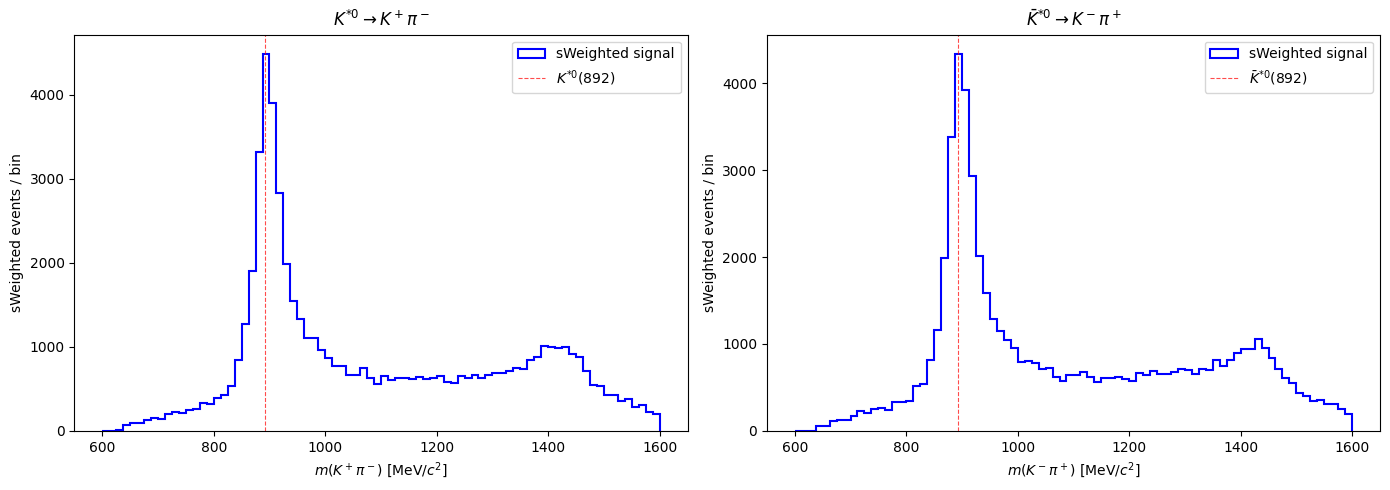
\includegraphics[width=0.95\textwidth]{../figures/exp_q5_kpi_sweighted.png}
\caption{sWeighted $m(K^+\pi^-)$ (left) and $m(K^-\pi^+)$ (right) distributions; dashed lines mark the $K^{*0}(892)$ mass.}
\label{fig:kpi_proj}
\end{figure}

\textbf{Other mass combinations.} The $m(K^+K^-)$, $m(\pi^+\pi^-)$
and same-sign $m(K^\pm\pi^\pm)$ distributions
(Figure~\ref{fig:other_proj_2body}) are broad and featureless, as
expected since these pairs originate from different $K^{*0}$ decays.
A ghost bump near 892~MeV in the same-sign pairs is a kinematic
reflection of the narrow $K^{*0}$.  The 3-body combinations
$m(K\pi\pi)$ and $m(KK\pi)$ (Figure~\ref{fig:other_proj_3body}) peak
near the kinematic endpoint set by $m_{B_s}$, with no narrow
resonant structures.

\begin{figure}[htbp]
\centering
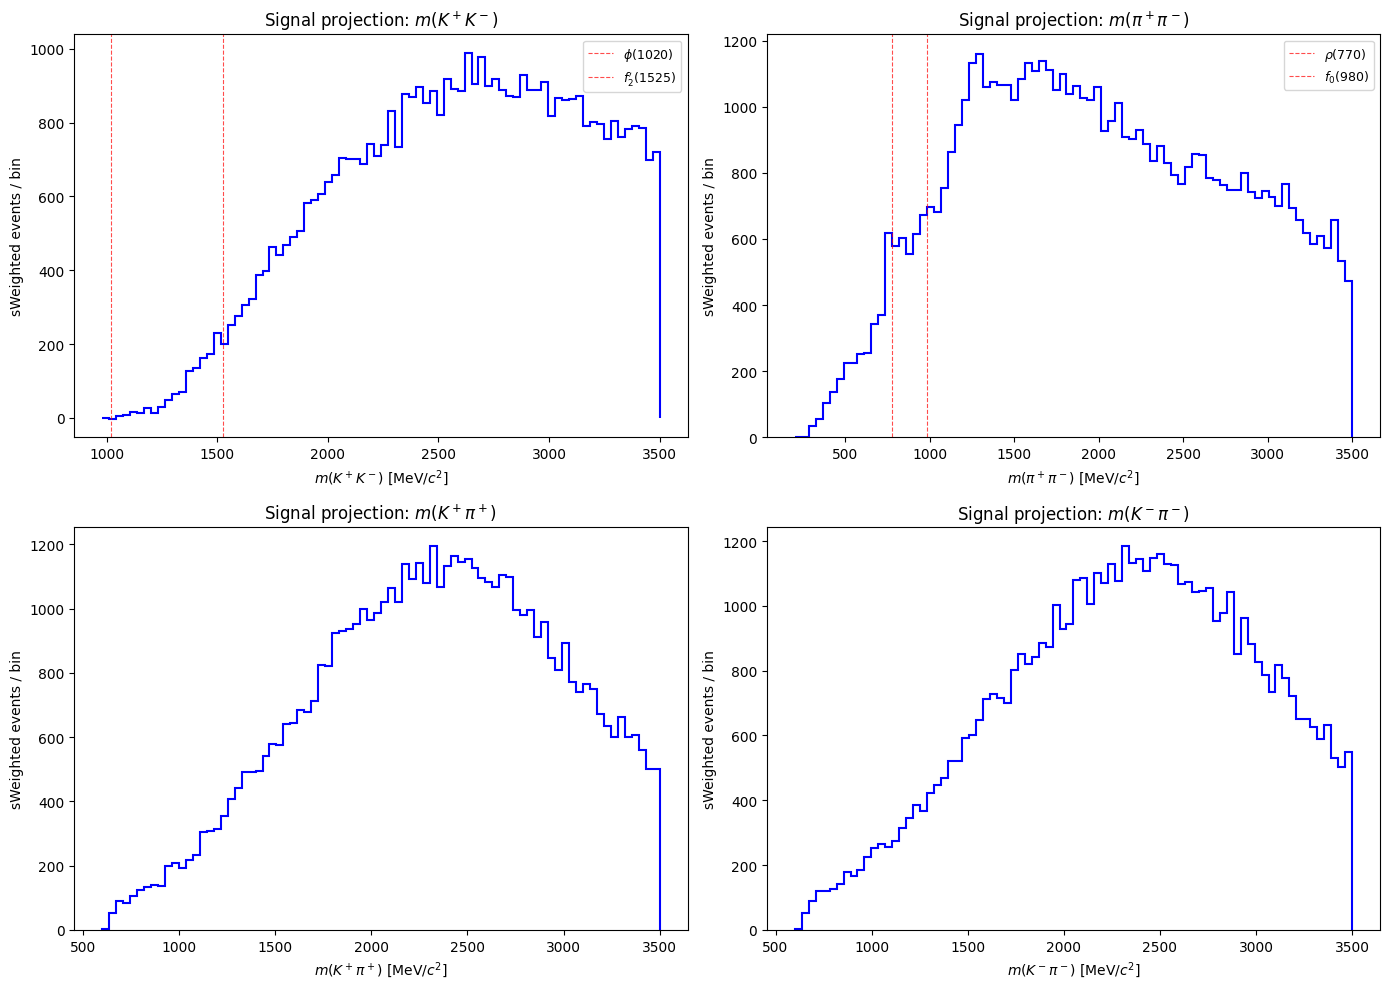
\includegraphics[width=0.8\textwidth]{../figures/exp_q5_other_sweighted_2-body.png}
\caption{sWeighted $m(K^+K^-)$, $m(\pi^+\pi^-)$, $m(K^+\pi^+)$, and $m(K^-\pi^-)$ distributions.}
\label{fig:other_proj_2body}
\end{figure}

\begin{figure}[htbp]
\centering
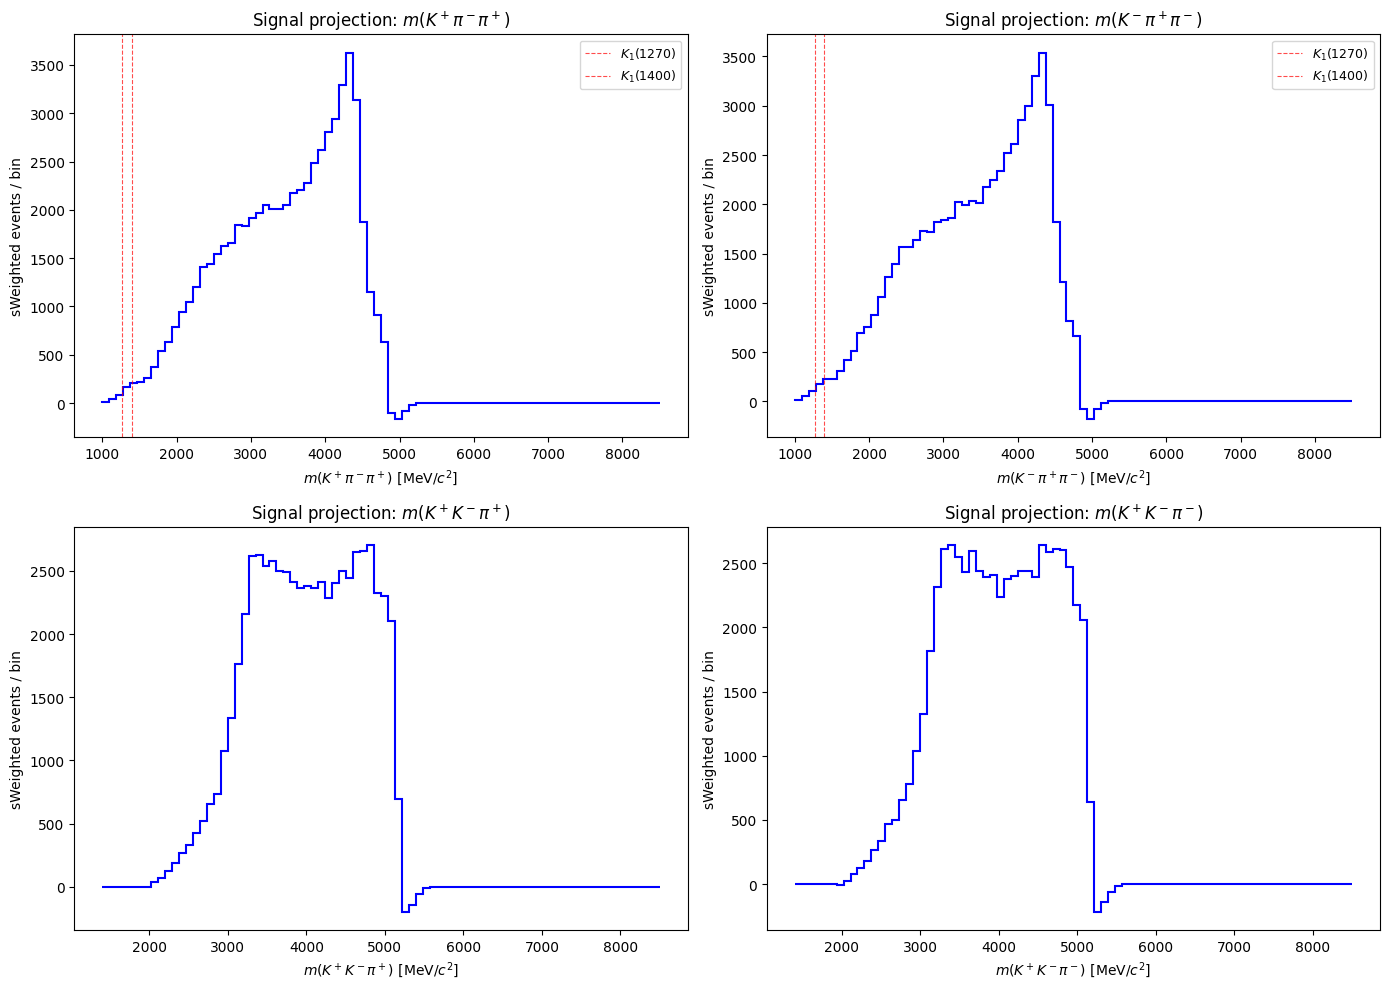
\includegraphics[width=0.8\textwidth]{../figures/exp_q5_other_sweighted_3-body.png}
\caption{sWeighted $m(K^+\pi^-\pi^+)$, $m(K^-\pi^+\pi^-)$, $m(K^+K^-\pi^+)$, and $m(K^+K^-\pi^-)$ distributions.}
\label{fig:other_proj_3body}
\end{figure}

\section{Summary (29 words)}

We isolated ${\sim}62{,}000$ $B_s^0 \to K^+\pi^-K^-\pi^+$ signal events using a BDT, PID cuts, and a $\phi$ mass veto. Signal-projected $K\pi$ distributions reveal dominant $K^{*0}(892)$ and secondary $K_2^*(1430)$ resonances.


\section*{Use of generative AI}
Claude (Anthropic) was used to assist with code development and
report writing. All outputs were reviewed and tested by the author,
who takes full responsibility for the final submission.

\begin{thebibliography}{99}

\bibitem{lhcb_kskpi} LHCb collaboration, R.~Aaij \textit{et al.}, ``Amplitude analysis of $B_s^0 \to K_S^0 K^\pm \pi^\mp$ decays,'' JHEP \textbf{06} (2019) 114, arXiv:1902.07955.

\bibitem{splot} M.~Pivk and F.~R.~Le~Diberder, ``sPlot: a statistical tool to unfold data distributions,'' Nucl.\ Instrum.\ Meth.\ A \textbf{555} (2005) 356, arXiv:physics/0402083.

\bibitem{iminuit} H.~Dembinski \textit{et al.}, ``iminuit -- A Python interface to Minuit2,'' \url{https://github.com/scikit-hep/iminuit}.

\end{thebibliography}

\end{document}